\documentclass[ignorenonframetext, professionalfonts, hyperref={pdftex, unicode}]{beamer}

\usetheme{Copenhagen}
\usecolortheme{wolverine}

%Packages to be included
%\usepackage{graphicx}

\usepackage[russian]{babel}
\usepackage[utf8]{inputenc}
\usepackage[T1]{fontenc}

%%\usepackage[orientation=landscape, size=custom, width=16, height=9.75, scale=0.5]{beamerposter}

\usepackage{textcomp}

\usepackage{beamerthemesplit}

\usepackage{ulem}

\usepackage{verbatim}

\usepackage{ucs}


\usepackage{listings}
\lstloadlanguages{bash}

\lstset{escapechar=`,
	extendedchars=false,
	language=sh,
	frame=single,
	tabsize=2, 
	columns=fullflexible, 
%	basicstyle=\scriptsize,
	keywordstyle=\color{blue}, 
	commentstyle=\itshape\color{brown},
%	identifierstyle=\ttfamily, 
	stringstyle=\mdseries\color{green}, 
	showstringspaces=false, 
	numbers=left, 
	numberstyle=\tiny, 
	breaklines=true, 
	inputencoding=utf8,
	keepspaces=true,
	morekeywords={u\_short, u\_char, u\_long, in\_addr}
	}

\definecolor{darkgreen}{cmyk}{0.7, 0, 1, 0.5}

\lstdefinelanguage{diff}
{
    morekeywords={+, -},
    sensitive=false,
    morecomment=[l]{//},
    morecomment=[s]{/*}{*/},
    morecomment=[l][\color{darkgreen}]{+},
    morecomment=[l][\color{red}]{-},
    morestring=[b]",
}

\author[Epam]{{\bf Epam}\\Low Level Programming Department}

%\institution[EPAM]{EPAM}
%\logo{\includegraphics[width=1cm]{logo.png}}


\title[binutils]{Binutils. Анализ исполняемого файла}

\begin{document}


%%%%%%%%%%%%%%%%%%%%%%%%%%%%%%%%%%%%%%%%%%%%%%%%%
%%%%%%%%%% Begin Document  %%%%%%%%%%%%%%%%%%%%%%
%%%%%%%%%%%%%%%%%%%%%%%%%%%%%%%%%%%%%%%%%%%%%%%%%

\begin{frame}
	\frametitle{}
	\titlepage
	\vspace{-0.5cm}
	\begin{center}
	%\frontpagelogo
	\end{center}
\end{frame}

\begin{frame}
	\tableofcontents
%	[hideallsubsections]
\end{frame}



%%%%%%%%%%%%%%%%%%%%%%%%%%%%%%%%%%%%%%%%%   
%%%%%%%%%% Content starts here %%%%%%%%%%
%%%%%%%%%%%%%%%%%%%%%%%%%%%%%%%%%%%%%%%%%
\mode<all>{%%

\begin{frame}
	\frametitle{Кого будем потрошить?}

	\begin{block}{Жертва обстоятельств}
		Для анализа понадобится пример из занятия по введению в gcc.\\
		Пример доступен по адресу:\\
		 \url{https://github.com/d4s/linux\_courses/tree/master/epam/examples/make/linking}
	\end{block}
\end{frame}
}

\section{Динамически связанные библиотеки}
\mode<all>{%%
%%

\begin{frame}
	\frametitle{Библиотеки и связи}

	\begin{block}{Утилита ldd}
		Просмотр списка библиотек от которых зависит программа.
	\end{block}

	\pause

	\begin{block}{Упражнение}
		\begin{enumerate}
			\item Запустить {\tt ldd main-A\_B main-B\_A}
			\item Заменить в {\tt Makefile} опцию {\tt -{}-no-as-needed} на {\tt -{}-as-needed}
				и перекомпилировать пример
			\item Повторить вызов {\tt ldd}, сравнить с предыдущим и сделать выводы
			\item Запустить {\tt ldd libtestb.so}
			\item Сравнить с выводом {\tt /usr/bin/java} и удивиться ;-)
		\end{enumerate}
	\end{block}

\end{frame}


}

\section{Структура elf}
\mode<all>{%%

\begin{frame}
	\frametitle{ABI исполняемых файлов в Linux}

	\begin{block}{Форматы исполняемых файлов}
		\begin{itemize}
			\item {\tt a.out} -- начало Unix
			\item {\tt COFF} -- Common Object File Format -- историческое продолжение {\tt a.out}
			\item {\tt ELF} -- Executable and Linkable Format -- настоящее Unix-like систем
		\end{itemize}
	\end{block}
\end{frame}

\begin{frame}
	\frametitle{ELF}
	\begin{columns}
		\column{0.5\textwidth}
			\begin{block}{Executable and Linkable Format}
				Файлы могут включать:
				\begin{itemize}
					\item Таблицу Program Header,  описывающую ноль или более сегментов
					\item Таблицу Section Header,  описывающую ноль или более секций
					\item Данные,  упомянутые в записях названных таблиц
				\end{itemize}
			\end{block}
		\column{0.5\textwidth}
			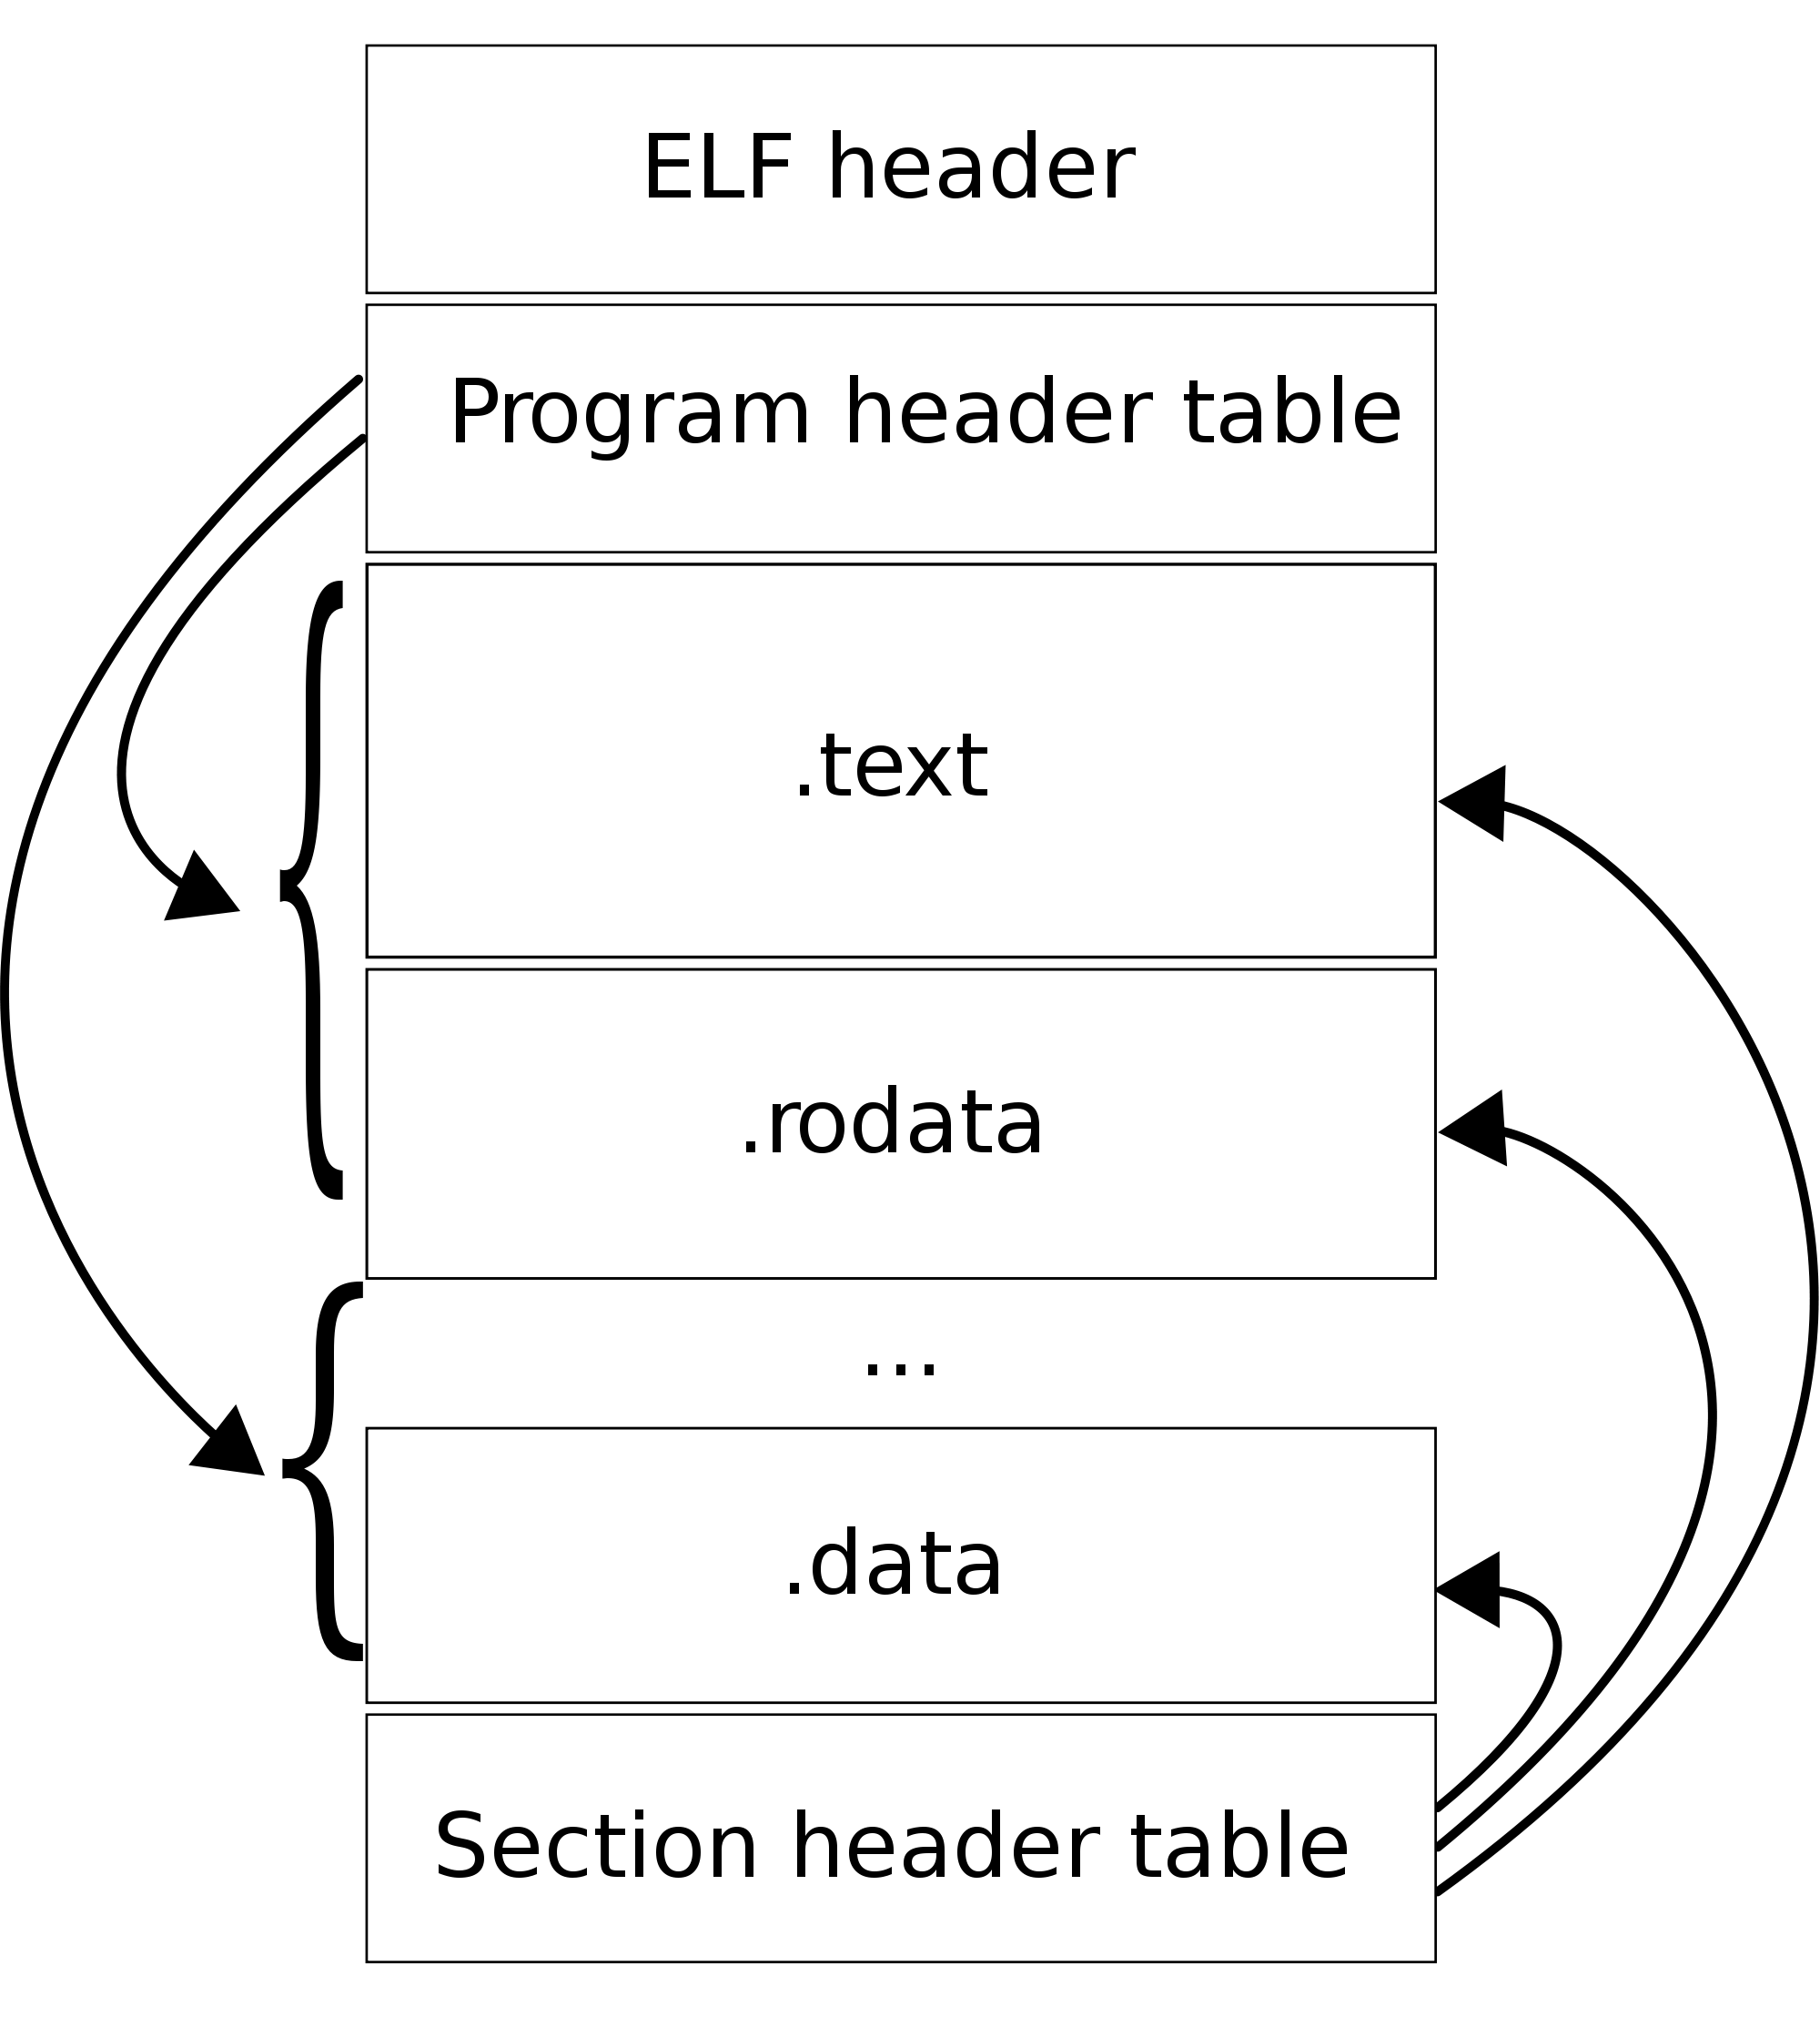
\includegraphics[height=0.8\textheight]{../../slides/elf-analysis/Elf-layout.png}
	\end{columns}
\end{frame}

\begin{frame}
	\frametitle{Структура ELF-файла}

	\begin{block}{readelf}
		Утилита для просмотра информации файлов в формате ELF.
	\end{block}

	\pause

	\begin{block}{Упражнение: просмотр программных заголовков}
		\begin{itemize}
			\item {\tt readelf -{}-file-header main-A\_B} -- интерпретация заголовка ELF-файла
			\item {\tt readelf -{}-sections main-A\_B} -- перечисление секций (для линковки)
			\item {\tt readelf -{}-segments main-A\_B} -- 
				перечисление программных сегментов (для исполнения)
			\item {\tt readelf -{}-symbols main-A\_B} -- список таблицы символов
		\end{itemize}
	\end{block}
\end{frame}

\begin{frame}
	\frametitle{Таблица символов}

	\begin{block}{strings}
		Утилита для получения символов из ELF-файла.
	\end{block}

	\begin{block}{nm}
		Утилита для получения символов из object файла.
	\end{block}

	\begin{block}{strip}
		Утилита для удаления символов из object файла.
	\end{block}
\end{frame}

\begin{frame}
	\frametitle{Таблица символов}

	\begin{block}{Упражнение}
		\begin{enumerate}
			\item {\tt strings main-A\_B}
			\item {\tt nm main-A\_B}
			\item {\tt nm -u main-A\_B}
			\item {\tt ls -l main-A\_B}
			\item {\tt strip main-A\_B}
			\item {\tt ls -l main-A\_B}
			\item {\tt nm main-A\_B}
			\item {\tt повторить предыдущее упражнение}
			\item Сделать выводы
		\end{enumerate}
	\end{block}

\end{frame}

}

\section{Binutils}
\mode<all>{%%
%% 

\begin{frame}
	\frametitle{objdump}

	\begin{block}{objdump}
		Утилита для просмотра информации по object файлам.
	\end{block}

	\pause

	\begin{block}{Упражнение}
		\begin{itemize}
			\item {\tt objdump -{}-file-headers main-A\_B} -- получить заголовок файла
			\item {\tt objdump -{}-section-headers main-A\_B} -- перечисление секций (для линковки)
			\item {\tt objdump -{}-syms main-A\_B} -- список таблицы символов
			\item {\tt objdump -{}-dynamic-syms main-A\_B} -- список динамических символов (как nm -u)
		\end{itemize}

	\end{block}
\end{frame}


\begin{frame}
	\frametitle{Дизассемблер objdump}

	\begin{block}{Упражнение: внутренниий мир программы}
		\begin{itemize}
			\item {\tt objdump -{}-disassemble main-A\_B} -- получить дизассемблированный файл
			\item {\tt objdump -{}-disassemble -j.text main-A\_B} -- 
				получить дизассемблированную исполняемую секцию {\tt .text}
			\item {\tt objdump -{}-disassemble -j.text -{}-file-offsets main-A\_B} -- 
				получить дизассемблированную исполняемую секцию {\tt .text} 
				и узнать где в файле располагаются инструкции
		\end{itemize}
	\end{block}
\end{frame}

\begin{frame}
	\frametitle{Что же наделал компилятор?}

	\begin{block}{Упражнение: анализируем вместе с исходником}
		\begin{itemize}
			\item Добавить в исходник {\tt main.c} объявление переменной и пустой цикл
			\item Добавить в {\tt Makefile} опции {\tt -g -O0}
			\item {\tt objdump -{}-source -{}-line-numbers main-A\_B}
			\item {\tt objdump -{}-source -{}-line-numbers -{}-file-offsets main.o}
			\item Изменить в {\tt Makefile} опцию {\tt -O0} на {\tt -O3}
			\item {\tt objdump -{}-source -{}-line-numbers -{}-file-offsets main.o}
			\item Сделать выводы ;-)
		\end{itemize}
	\end{block}
\end{frame}

}

\end{document}
